\section{Introduction}

In this project, I will investigate options for synthesizing digital
circuits without clocks. A prerequisite for such a solution is a
high-level language that ultimately can create circuits for
implementation in silicon. I will also implement a circuit for the
\nomenclature{AES}{Advanced Encryption Standard} Advanced Encryption
Standard with one of these technologies, and attempt to identify
challenges and potential with such a solution.

One major assumption in the majority of digital
\nomenclature{VLSI}{Very-Large-Scale Integration} VLSI circuits
produced today, is the notion of a discrete and common time. This is
provided by one or more clocks. This is an important simplification
that makes reasoning about digital circuits easier. However, as
circuits grow in size and complexity, it is ``well known''
\cite[pp. 5]{sparso} that the task of providing a clock-signal
simultaneously to all flip-flops in the circuit becomes an
increasingly difficult task.

\begin{figure}[htbp]
  \centering
  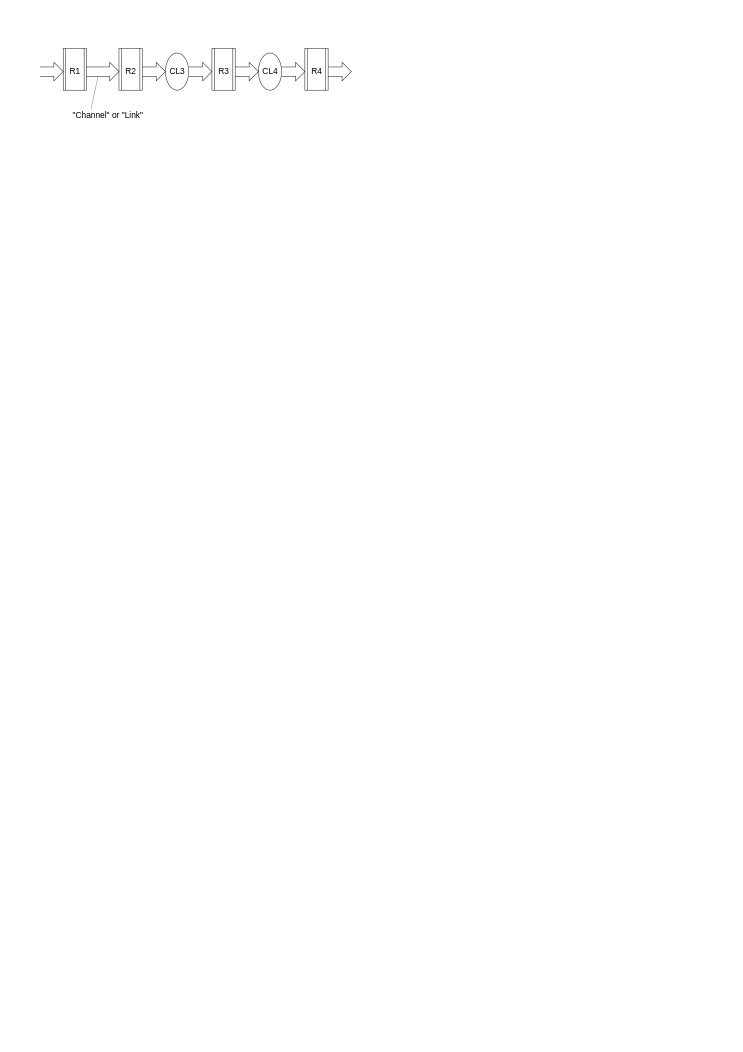
\includegraphics{flow.pdf}
  \caption{An abstract view of a digital circuit with registers and
    combinational logic (CL). Figure from \cite{sparso}.}
  \label{fig:flow}
\end{figure}

When designing a digital circuit for solving a computable problem, it
is usual to split the problem into multiple combinational circuits
with memory elements interspersed as shown in
figure~\ref{fig:flow}. The value of a memory element is then
determined by the value of the previous memory element modified by a
combinational circuit. However, this combinational circuit has a
non-zero delay, and there is usually no reliable way to determine when
the output value has been completely calculated. With clocked
circuits, the completeness of a calculation is guaranteed by assuming
worst case conditions and setting the clock-frequency accordingly.

As digital circuits have grown, designing have increasingly become a
problem of managing complexity \cite{flynn2009deep}. To make
specifications with varying levels of abstractions in hardware
description languages, such as VHDL and Verilog, is crucial for
digital designers to manage complexity.

The motivation for investigating clockless is that the clock, while
conceptually simple, imposes increased complexity when the circuits
grow; the clock can ultimately end up complicating the design instead
of simplifying it. Clockless circuits also have different and
interesting characteristics: 
\begin{itemize}

\item The clock in a conventional design is one of the main
  contributors to power-consumption \cite{tiwari1998reducing}.

\item The simultaneity of the clock makes the circuits exhibit
  noticeable spikes in the electromagnetic spectrum.

\item The whole problem of clock domain crossing is sidestepped,
  allowing a higher degree of modularity and reusability.

\item Clockless designs are more robust to variations in process
  technologies and operating conditions. The speed of clockless
  circuits automatically adapts to doping variations, temperature and
  voltage.

\item Clockless circuits does not require massive, ``cheap'', metallic
  fan-outs (the clock) provided by the silicon-technology today. Future
  technologies for implementing logic, such as rapid single flux
  quantum, may not provide a similar simple fan-out mechanism \cite{rapid}.
\end{itemize}

When mapping high-level description hardware-languages to silicon,
there must also be implemented a form of completion-detection for the
combinational circuits to drive the memory-elements instead of the
clock. I will outline some of these techniques in this project.

A major issue with clockless circuits, is that it is a relatively
young discipline without an industry-wide adoption, or widespread
experience. Production testing is essential for mass-production, and
while important work have been done on testing and clockless
circuits\cite{fullscan}, it is not widely available in all
design-flows.

As practical work, I will attempt to implement a clockless Advanced
Encryption Standard (AES)\cite{rijandael} encryption module to explore
high level clockless design. The AES is choosen because it is a well
defined standard, and has a reasonable complexity for this
project. While previous work on clockless AES\cite{claes} have focused
on security, I will in this project mainly explore the AES to survey
clockless high-level design.

